\documentclass[12pt]{article}
\usepackage{subfig}
\usepackage{tikz}
\usepackage{mathtools}
\usepackage{enumitem}
\usepackage{amsthm,amsfonts}
\newcommand{\bmmax}{0}
\newcommand{\hmmax}{0}
\usepackage{amsmath,amssymb,bm,bbm}
\usepackage{relsize}


\usetikzlibrary{arrows,calc,patterns,angles,quotes,3d,arrows.meta,decorations.pathreplacing}

\usepackage{anyfontsize}
\usepackage[left=1.45in,right=1.45in,top=0.8in,bottom=1.1in,footskip=.5in]{geometry}
\usepackage[stretch=10,shrink=10]{microtype}
% Import \ast symbol from cm
\DeclareFontFamily{OMS}{kstcmsy}{\skewchar\font48 }
\DeclareFontShape{OMS}{kstcmsy}{m}{n}{%
      <5><5.5><6><7><8><9><10>gen*cmsy%
      <10.5><10.95><12><14.4><17.28><20.74><24.88>cmsy10%
      }{}
\DeclareFontShape{OMS}{kstcmsy}{b}{n}{%
      <5><5.5><6><7><8><9>gen*cmbsy%
      <10><10.95><12><14.4><17.28><20.74><24.88>cmbsy10%
      }{}
\DeclareSymbolFont{kstsymbols}{OMS}{kstcmsy}{m}{n}

\DeclareFontFamily{OML}{kstcmm}{\skewchar\font127 }
\DeclareFontShape{OML}{kstcmm}{m}{it}%
     {<5><5.5><6><7><8><9>gen*cmmi%
      <10><10.5><10.95>cmmi10%
      <12><14.4><17.28><20.74><24.88>cmmi12%
      }{}
\DeclareFontShape{OML}{kstcmm}{b}{it}{%
      <5><5.5><6><7><8><9>gen*cmmib%
      <10><10.95><12><14.4><17.28><20.74><24.88>cmmib10%
      }{}
\DeclareFontShape{OML}{kstcmm}{bx}{it}%
   {<->ssub*cmm/b/it}{}
\DeclareSymbolFont{kstletters}     {OML}{kstcmm} {m}{it}
\DeclareMathSymbol{\ast}{\mathbin}{kstsymbols}{"03}
\DeclareMathSymbol{\star}{\mathbin}{kstletters}{"3F}

\renewcommand{\rmdefault}{zpltlf} % Roman font for use in math mode
\usepackage{newpxmath}
\usepackage{newpxtext}

\setlength{\parindent}{1.8em}
\renewcommand{\baselinestretch}{1.4}


% ----------------- commands --------------------
\renewcommand*{\vec}[1]{\mathbf{#1}}
\newcommand{\gvec}[1]{\bm{#1}}

\DeclareMathOperator{\fft}{fft}
\DeclareMathOperator{\tr}{tr}
\DeclareMathOperator{\atantwo}{atan2}
\DeclareMathOperator{\Cov}{Cov}
\DeclareMathOperator{\lcm}{lcm}
\DeclareMathOperator{\Aut}{Aut}
\DeclareMathOperator{\Inn}{Inn}
\DeclareMathOperator{\orb}{orb}
\DeclareMathOperator{\stab}{stab}
\DeclareMathOperator*{\argmax}{arg\,max}
\DeclareMathOperator*{\argmin}{arg\,min}

\newcommand*{\R}{\ensuremath{\mathbb{R}}}
\newcommand*{\N}{\ensuremath{\mathbb{N}}}
\newcommand*{\Z}{\ensuremath{\mathbb{Z}}}
\newcommand*{\Cplx}{\ensuremath{\mathbb{C}}}
\newcommand*{\Q}{\ensuremath{\mathbb{Q}}}
% transpose
\newcommand*{\Trans}{\ensuremath{{\mkern-1.5mu\mathsf{T}}}}
\newcommand{\Conj}[1]{\overline{#1}}
\newcommand{\Hermconj}{\ensuremath{\mathsf{H}}}
\newcommand{\One}{\ensuremath{\mathlarger{\mathbbm{1}}}}


\title{\vspace{-7.5ex}\textbf{\Large CSE546 Homework 1}\vspace{-1.7ex}}
\author{Chuanmudi Qin}
\date{\vspace{-1ex}April 21, 2020\vspace{-5ex}}

\begin{document}
\maketitle
\section*{A0}
1.  \\
$\bullet$ Bias: measures the square differences between predicted value with true value.In this context: mean square of the difference between the true mean and Expected value of Sample mean under the trained $\widehat{f_{\mathcal{D}}}$\\ 
$\bullet$  Variance:measures how spread out the predicted values are from the true mean. In this context:  the expectation of the square differences between predict value under the traine $\widehat{f_{\mathcal{D}}}$ and the expectation of values under all trained $\widehat{f_D}$\\ 
$\bullet$ with a learned/trained function $\widehat{f_D}$, the bias decrease as the complexity of the function increase, whereas the variance increase as complexity increase. the total error which is the sum of the two first decrease then increase. The goal is to find a appropriate complexity that balance bias and viariance so that the total error is minimized.\\

\noindent 2. \\
$\bullet$ with a learned/trained function $\widehat{f_D}$, the bias decrease as the complexity of the function increase, whereas the variance increase as complexity increase.\\

\noindent 3. False \\

\noindent 4. False \\

\noindent 5. False \\

\noindent 6. Training set. \\
$\bullet$ testing set should not be used until we are ready to report how good the learned functions are doing.\\

\noindent 7. False \\
$\bullet$ usually it provides a underrestimate of the true error  
\newpage
\section*{A1}
Before answering $(a)$,$(b)$,$(c)$, I would first want to derive the formula: \\
\[
\begin{aligned}
        P(X_1 =x_i, X_2= x_2, ...,X_n=x_n) &= \prod_{i=1}^{n}P_{oi}(x_i | \lambda) = e^{-\lambda n} \prod_{i=1}^{n} \frac{\lambda^{x_i}}{x_i!}\\
        \widehat{\lambda_{MLE}}      &= \argmin_{\lambda} [e^{-\lambda n} \prod_{i=1}^{n} \frac{\lambda^{x_i}}{x_i!}]\\
                  &=\argmin_{\lambda}  [ log (e^{-\lambda n} \prod_{i=1}^{n} (\frac{\lambda^{x_i}}{x_i!})] \\
                   &=\argmin_{\lambda}  [ log (e^{-\lambda n}) + log( \prod_{i=1}^{n} (\frac{\lambda^{x_i}}{x_i!})] \\
                   &= -\lambda n + \sum_{n=1}^{n} log(\frac{\lambda^{x_i}}{x_i !})\\
                   &= -\lambda n + \sum_{n=1}^{n} (log(\lambda^{x_i} - log(x_i !)) 
\end{aligned}
\]

Solve the above by taking derivatie and set to 0: \\
\[
\begin{aligned}
        \frac{d}{d\lambda} ( -\lambda n + \sum_{n=1}^{n} (log(\lambda^{x_i} - log(x_i !)) ) &=  -n + \sum_{i=1}^{n} \frac{x_i}{\lambda} = 0 \\ 
        \lambda &=\frac{ \sum_{i=1}^{n} x_i}{n} 
\end{aligned}
\]
\begin{proof}
        (a) \\ 
        following the above derivation: \\
        $$  \lambda =\frac{ \sum_{i=1}^{5} x_i}{5} $$ 
\end{proof}
\begin{proof}
        (b) \\ 
        following the above derivation: \\
        $$  \lambda =\frac{ \sum_{i=1}^{6} x_i}{6} $$ 
\end{proof}

\begin{proof}
        (c) \\ 
        following the above derivation: \\
        $$  \lambda =\frac{ \sum_{i=1}^{5} x_i}{5} = \frac{6}{5} $$ 
        $$  \lambda =\frac{ \sum_{i=1}^{6} x_i}{6} =\frac{10}{6}= \frac{5}{3}  $$ 
\end{proof}
\newpage

\section*{A2}
According the the spec, we know that: $P(X_i=x_i) = \frac{1}{theta}$
$$P(\mathcal{D} | \theta) = P(X_1=x_1, X_2=x_2,...,X_n=x_n ) = \frac{1}{\theta^n}$$
$$\frac{d}{d\theta}log(P(\mathcal{D} | \theta)) = -\frac{n}{\theta}$$
Because $\theta$ is always greater than 0, $-\frac{n}{\theta}$ is less than 0, we know that $P(\mathcal{D} | \theta)$ is monotonically decreasing. Given the observations: 
$$\widehat{\theta_{MLE}} =max(x_1,x_2,x_3,...,x_n) $$

\newpage

\section*{A3}
\begin{proof}
        (a).\\
        \[
\begin{aligned}
        E_{train}[\widehat{\epsilon}_{train}(f) ] &= E_{train}[\frac{1}{n} \sum_{(x_i,y_i)} (f(x_i)-y_i)^2 ] =[\frac{1}{n} \sum_{(x_i,y_i)} E_{train}(f(x_i)-y_i)^2 ]  \\
                                                  &= \int_{(x,y)\in training}\frac{1}{n} \sum_{(x,y)} (f(x_i)-y_i)^2  P(x_1,y_1,x_2,y_2...)d\mathbf{x}d\mathbf{y}\\ 
                                                  &(i.i.d)=  \int_{(x,y)}\frac{1}{n} \sum_{(x,y)} (f(x_i)-y_i)^2  P(x_1,y_1)P(x_2,y_2)...d\mathbf{x}d\mathbf{y}\\ 
                                                  &=  \frac{1}{n} \sum_{(x,y)} (f(x_i)-y_i)^2  \int_{x_1,y_1} \int_{x_2,y_2}...\int_{x_n,y_n} P(x_1,y_1)P(x_2,y_2)...d\mathbf{x}d\mathbf{y}\\ 
                                                  &=  \frac{1}{n} n \int_{x_1,y_1}   (f(x_i)-y_i)^2  P(x_i,y_i)dx_idy_i\\ 
                                                  & = E_{(x,y) \in \mathcal{D}} [(f(x)-y)^2] = \epsilon(f)
\end{aligned}
        \]
in a similar manner, we can prove $E_{test}[\widehat{\epsilon}_{tet}(f)] = \epsilon(f)$ \\ 

\noindent for a unbiased estimator $\widehat{f}$, it can be shown with a similar step as above that: $E_{test}(\epsilon(\widehat{f})) = \epsilon(\widehat{f})$. This equality holds because $\widehat{f}$ is trained with training set and it is independent with the test set.
\end{proof}

\begin{proof}
        (b)\\
        The equality does not hold. \\
        The unbiased estimator $\epsilon(\widehat{f})$ is obtained from the training set. Therefore the training error $E_{train}[\epsilon_{train}(\widehat{f})]$ is potentially underrestimate the True error.  
\end{proof}

\begin{proof}
        (c)\\
use a similar logic as example provided in the hint and total law of expectation: 
$$E_{train} [\widehat{e}(\widehat{f}_{train})] =\sum_{f \in \mathcal{F}}E_{train}[\widehat{\epsilon}_{train}(\widehat{f}_{train} |f)] *P_{train}(\widehat{f}_{train} = f)  $$
from the given hint in part (c): $$E_{train,test} =\sum_{f}E_{test}[\widehat{\epsilon_{test}}\widehat(f)] *P_{train}(\widehat{f}_{train} = f)  $$\\
by part (a), I know the followig:
 $$\sum_{f}E_{test}[\widehat{\epsilon_{test}}\widehat(f)] *P_{train}(\widehat{f}_{train} = f) = \sum_{f}E_{test}[\epsilon(f)] *P_{train}(\widehat{f}_{train} = f)$$ 
 we know that since $\widehat{f}$ is not independent from training set, $$\epsilon_{train}(\widehat{f}_{train}) < \epsilon(f)$$ 
Hence,
$$\sum_{f \in \mathcal{F}}E_{train}[\widehat{\epsilon}_{train}(\widehat{f}_{train} |f)] *P_{train}(\widehat{f}_{train} = f) \leq \sum_{f}E[{\epsilon}(f)] *P_{train}(\widehat{f}_{train} = f)  $$
$$ E_{train} [\widehat{e}(\widehat{f}_{train})] \leq  E_{train,test} [\widehat{\epsilon}_{test}(\widehat{f}_{train})]$$
\end{proof}

\newpage

\section*{B1}
\begin{proof}
        (a)\\
        Suppose n is the size of the data set. In this specific question, when m is low, the estimator $f$ will try fit every single point onto the curve. When $m=n$, the estimator will be the average value of all n data points(i.e a constant)for all predictions. \\
        Therefore, intuitively, I would expect variance to grow when m is small, since this will be the situation where overfitting happens. and variance to be lower if m is large. And bias will be small if m is small, and it would grow as m gets large. 
\end{proof}
\begin{proof}
        (b)\\
        \[
\begin{aligned}
      \star =  & \frac{1}{n} \sum_{i=1}^{n} (E[\widehat{f_m}(x_i) - f(x_i))^2\\
       &=  \frac{1}{n} \sum_{i=1}^{n} (E[\frac{1}{m}\sum^{\frac{n}{m}}_{j=1} \sum_{k=(j-1)m+1}^{jm} y_k \mathbbm{1}\{x_i \in (\frac{(j-1)m}{n}, \frac{jm}{n})\} ]- f(x_i))^2\\
       &=  \frac{1}{n} \sum_{i=1}^{n} (E[\frac{1}{m}\sum^{\frac{n}{m}}_{j=1} \sum_{k=(j-1)m+1}^{jm} y_k \mathbbm{1}\{x_i \in (\frac{(j-1)m}{n}, \frac{jm}{n})\} ]- f(x_i))^2\\
       &=  \frac{1}{n} \sum_{i=1}^{n} (\frac{1}{m}\sum^{\frac{n}{m}}_{j=1} \sum_{k=(j-1)m+1}^{jm}E[ y_k \mathbbm{1}\{x_i \in (\frac{(j-1)m}{n}, \frac{jm}{n})\} ]- f(x_i))^2 \\
\end{aligned}
        \]
        realizing, for every fixed i the expectation can be rewritten as: 
\[
\begin{aligned}
        & E[ y_k \mathbbm{1}\{x_i \in (\frac{(j-1)m}{n}, \frac{jm}{n})\} ] = \begin{cases}
                E[f(x_k)] + \epsilon  = f(x_k) , \qquad x_i \in (\frac{(j-1)m}{n}, \frac{jm}{n})\\ 
                0
        \end{cases}\\
        \star &=  \frac{1}{n} \sum_{i=1}^{n} (\frac{1}{m}\sum^{\frac{n}{m}}_{j=1} \sum_{k=(j-1)m+1}^{jm}f(x_k) \mathbbm{1}\{x_i \in (\frac{(j-1)m}{n}, \frac{jm}{n})\}- f(x_i))^2 \\
              &=  \frac{1}{n} \sum_{i=1}^{n} (\sum_{j=1}^{\frac{n}{m}} \bar{f}^{(j)}  \mathbbm{1}\{x_i \in (\frac{(j-1)m}{n}, \frac{jm}{n})\}- f(x_i))^2 \\
\end{aligned}
\]
and realize that for every i, there is only one none-zero term inside of the square(because every i can only belongs to 1 interval), but every m iteration of the outter sum share one function value. Therefore, we can exchange the orders of the sums: \\
$$\star  =  \frac{1}{n} \sum_{j=1}^{\frac{n}{m}} \sum_{i= (j-1)m}^{jm} (\bar{f}^{(j)} - f(x_i)^2 $$
\end{proof}

\begin{proof}
        (c)\\
        \[
\begin{aligned}
        \star = E[\frac{1}{n} \sum_{i=1}^{n} (\widehat{f}_m(x_i) - E[\widehat{f}(x_i)])^2 ] 
\end{aligned}
        \]
        due to it is very tedious to type out and the process is exactly the same as part(b), I will skip the expanding $\widehat{f}_m(x_k) $ part. The logic follows (b)
        
        \[
\begin{aligned}
        \star &=E[\frac{1}{n} \sum_{i=1}^{n} (\sum_{=1}^{\frac{n}{m}}c_j \mathbbm{1}\{x_i \in (\frac{j-1}{m}, \frac{jm}{m})\})^2 - E[\sum_{j=1}^{j=\frac{n}{m}} c_j x \in (\frac{j-1}{m}, \frac{jm}{m})]]\\
              &(\text{reasoning is the same as (b)})\\
         &= \frac{1}{n} \sum_{j=1}^{\frac{n}{m}}\sum_{i=j(m-1)}^{mj} E[c_j- E[c_j]^2]
\end{aligned}
        \]
        for a fixed j, the inner yields the same values for very i: \\
        \[
\begin{aligned}
        * &= \frac{1}{n} \sum_{j=1}^{\frac{n}{m}} m E[(c_j- E[c_j])^2] \\ 
        * & =  \frac{1}{n} \sum_{j=1}^{\frac{n}{m}} m E[(c_j- \frac{1}{m} \sum_{k=(j-1)m}^{jm} f(x_k)) ^2]\\
          &= \frac{1}{n} \sum_{j= 1}^{\frac{n}{m}} m E[(c_j-\bar{f}^{(j)})^2]
\end{aligned}
        \]
To prove the second equality : \\ 
\[
\begin{aligned}
        *&= \frac{1}{n} \sum_{j= 1}^{\frac{n}{m}} m E[(\frac{1}{m}\sum_{m(j+1)}^{jm} y_i -\frac{1}{m}\sum_{j(m-1)}^{jm} f(x_i))^2]\\
         &=m *\frac{1}{n} *\frac{1}{m^2}  \sum_{j= 1}^{\frac{n}{m}} \sum_{m(j+1)}^{jm}  E[(y_i - f(x_i))^2]\\
          & = \frac{1}{mn} * n\sigma^2
\end{aligned}
\]
\end{proof}

\begin{proof}
        (d).\\
        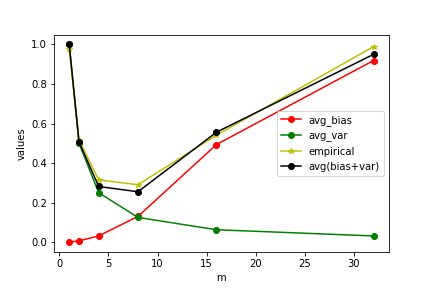
\includegraphics{../code/B1.png}
\end{proof}

\begin{proof}
        (e).\\
        recall the average bias is :
        $$\star = \frac{1}{n} \sum_{j=1}^{\frac{n}{m}}\sum_{i = (j-1)m+1}^{mj}(f^{(j)} - f(x_i))^2$$
        From the hint given, it can be ovserved that the quatity of $(f^{(j)} - f(x_i))^2$ is bounded for fixed $j$: 
        \[
        \begin{aligned}
                f^{(j)} & \leq  \max_{i \in ((m-1)j+1,mj) } f(x_i)\\
                f(x_i) & \geq   \min_{i \in ((m-1)j+1,mj) } f(x_i)\\
        (f^{(j)} -f(x_i) )^2 &\leq    |f^{(j)} -f(x_i) |^2  = (\frac{L}{n}|i-j|)^2  \leq  (\frac{L}{n}m)^2 
\end{aligned}
\]
Hence the inner sum is summing across constant: \\
\[
\begin{aligned}
        \star  \leq  \frac{1}{n} \sum_{j=1}^{\frac{n}{m}}\sum_{i = (j-1)m+1}^{mj} \frac{L^2 m^2}{n^2} = \frac{1}{n}*\frac{n}{m}*m *\frac{L^2 m^2}{n^2} = O(\frac{L^2m^2}{n^2})
\end{aligned}
\]\\

To minimize the total error that is of $O(\frac{L^2m^2}{n^2} + \frac{\sigma^2}{m})$, 

\[
\begin{aligned}
        & \frac{d}{dm}(\frac{L^2m^2}{n^2} + \frac{\sigma^2}{m})  = \frac{2L^2m}{n^2} - \frac{\sigma^2}{m^2} \implies m = (\frac{n^2\sigma^2}{2L^2})^{\frac{1}{3}}
\end{aligned}
\]\\
Plug this back into the total error: 
$$O(\frac{L^2m^2}{n^2} + \frac{\sigma^2}{m})=O(\frac{L^2((\frac{n^2\sigma^2}{2L^2})^{\frac{1}{3}}
)^2}{n^2} + \frac{\sigma^2}{(\frac{n^2\sigma^2}{2L^2})^{\frac{1}{3}} 
})$$
\end{proof}

\newpage
\section*{A4 A5 graphs}
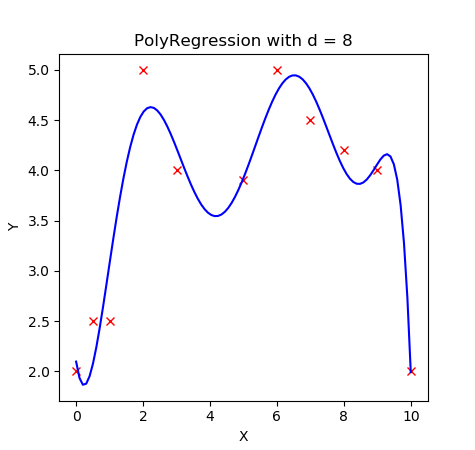
\includegraphics{../code/A4.png}\\
\newpage
the graph should be correct it is just I changed plt.xlim()\\ 
\noindent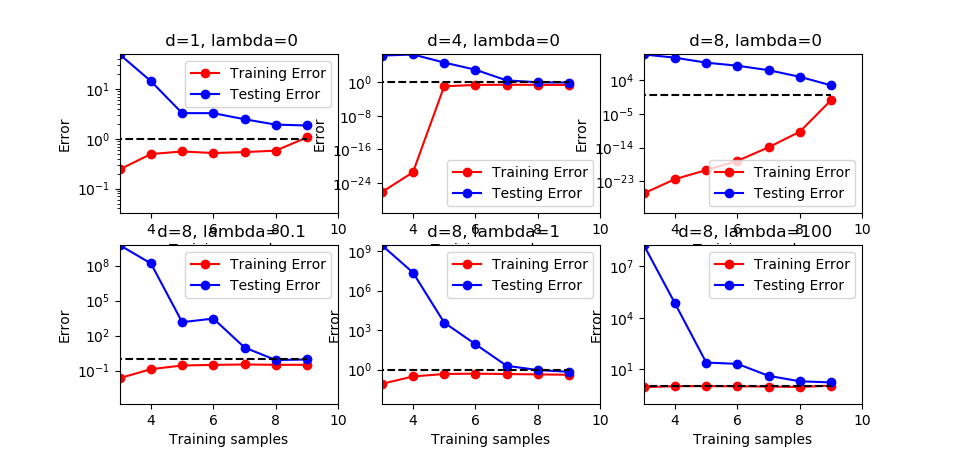
\includegraphics[width =15cm, height = 10cm]{../code/A5.png}
\newpage
\section*{A6}
\begin{proof}
        (a)\\
\[
        \begin{aligned}
             \frac{d}{d\mathbf{w}}   \star &=\frac{d}{d\mathbf{w}} \sum_{j=0}^{k} [||Xw_j - Yej||^2 + \lambda ||w_j||^2] \\    
                &\text{then every entry of the gradient is: }\\
             \frac{d}{dw_j} * &= \frac{d}{dw_j}[||Xw_j - Yej||^2 + \lambda ||w_j||^2] \\    
                &\text{using chain rule }\\
             \frac{d}{dw_j} * &= 2(Xw_j-Ye_j)^{T} X +2\lambda w_j\\ 
                              &\text{set it to zero and solve: }\\
             X^TXw_j &+ \lambda I w_j = X^TYe_j\\
             w_j &= ( X^TX + \lambda I)^{-1} X^{T}Ye_j\\
             \text{Hence: }\\
W &= ( X^TX + \lambda I)^{-1} X^{T}Y
        \end{aligned}
\]
\end{proof}

\begin{proof}
        (b).\\
        (code attached on the next pages)\\
        after standardizing, the the training error is : 0.14226666666666668, the testing error is : 0.13970000000000002
\end{proof}

\newpage
\section*{B1}

\begin{proof}
        (a).\\
        \includegraphics{../python-mnist/B2.png}
\end{proof}

\begin{proof}
        (b).\\

        the testing error is : 0.013581015157406196\\
the 95\% confidence interval is ( 0.8939189848425939 , 0.9210810151574063 )\\
Justification: \\
Realizing with a $\delta=0.05$ and 10000 records in total determind, the bounds can be calculated as the following: \\
$$z= \sqrt{\frac{(b-a)log(\frac{2}{\delta})}{2m}} =  \sqrt{\frac{log(\frac{2}{.05})}{2*10000}} = 0.013581015157406196 $$

The way we should interpret Hoeffding’s inequality is: The square differences between predicted value and true value can be seen as a random variable for each pixel. Then, the true error $\mu$ can be calculated from the $$\frac{1}{10000}\sum_{m=1}^{m=10000} (error_i) \pm z$$
Therefore, we get the interval:\\ 
$$( 0.8939189848425939 , 0.9210810151574063 )$$
\end{proof}
\end{document}
\section{Chapter 1}
\subsection*{Problem 1}

\begin{enumerate}[label=\roman*)]
  \item $a \in \Z$
  \item $A^\Trans = A$
  \item $A\vec{v} = \lambda \vec{v}$
  \item $\One$
\end{enumerate}
pupupu $|a|=15$, pupupupu.
